\documentclass{beamer}

\usetheme{CambridgeUS} %feel free to adjust the theme

\title{Evaluating Urban Green Space}
\subtitle{MACS 30200 Project}
\author{Kuang Sheng}
\institute{University of Chicago}
\date{\today}


\begin{document}

\begin{frame}
\titlepage
\end{frame}

\begin{frame}
\frametitle{Outline}
\tableofcontents
\end{frame}

\section{Introduction}
\subsection{Background Overview}

\begin{frame}
\frametitle{Background Overview}
\begin{figure}[h]
  \centering
  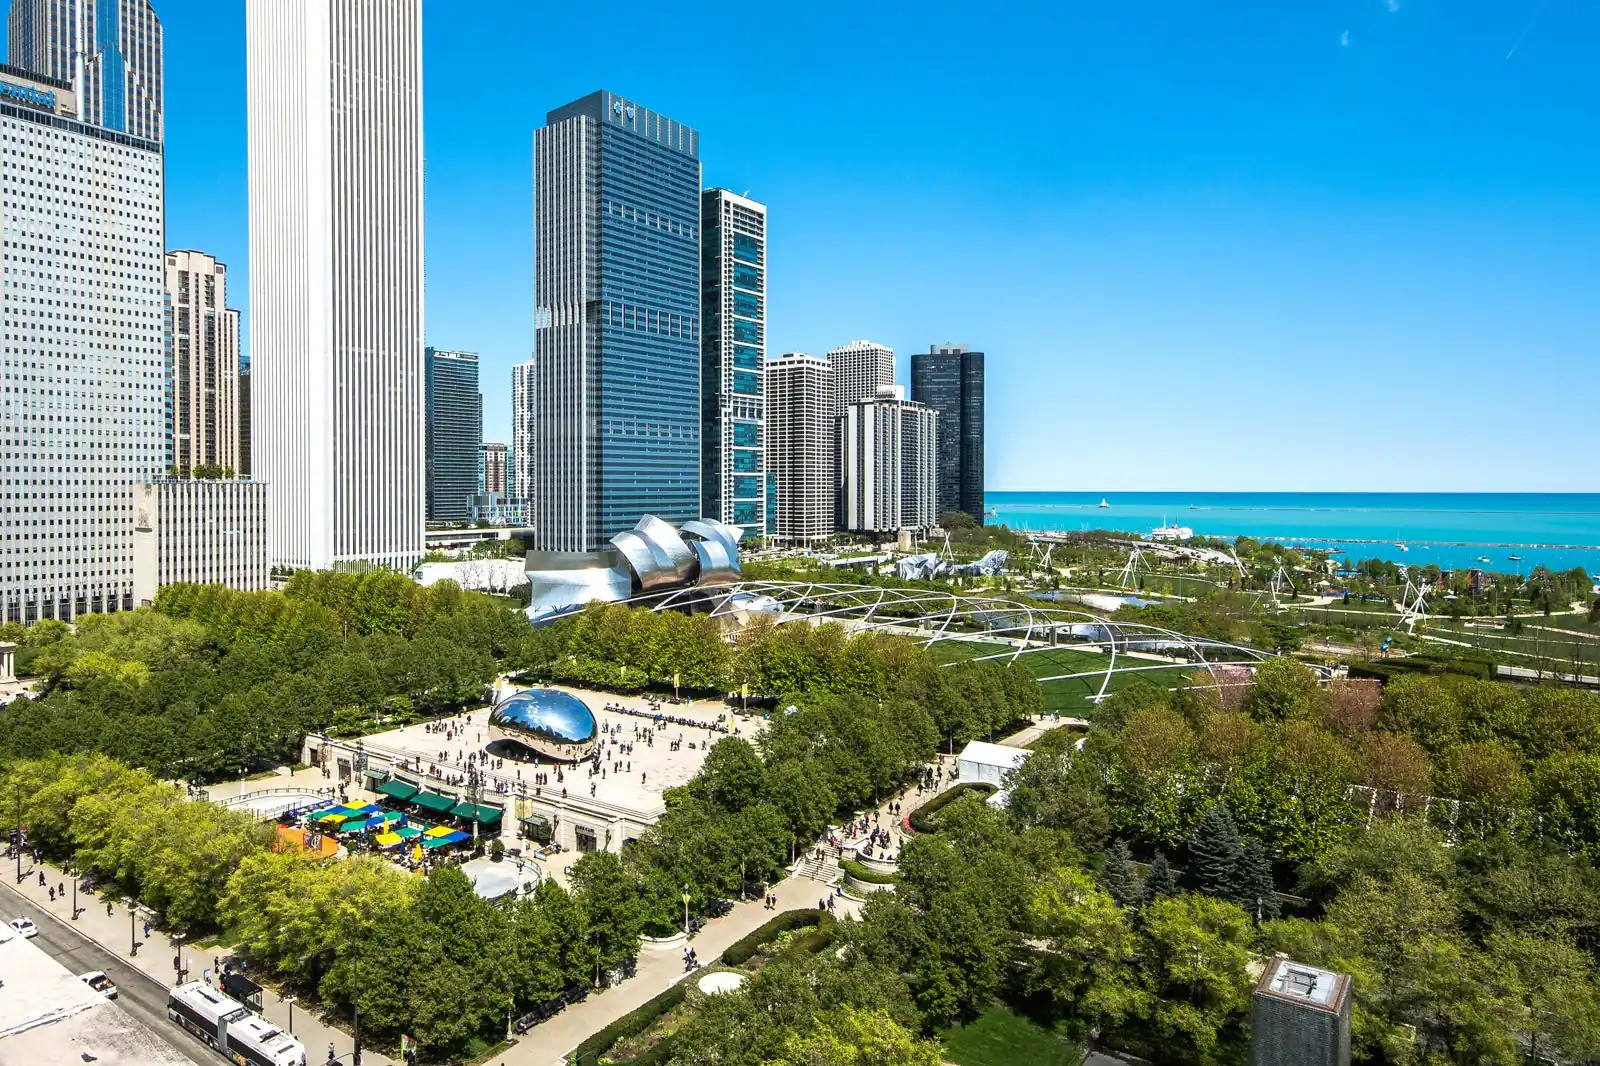
\includegraphics[width=0.35\textwidth]{Visual/MPark.jpg}
\end{figure}
In previous studies, Urban Green Space (UGS) shows continuous influence on urban residents’: 
\frametitle{Overview}
\begin{itemize}
    \item Well-Being
    \item Economic Benefits
    \item Social Equality
\end{itemize}
Studying the value of UGS in different urban environments can advocate a better urban environment, generate economic benefits, and alleviate urban segregation.
\end{frame}

\subsection{Literature}

\begin{frame}
\frametitle{Literature}
\begin{itemize}
    \item Previous research: utilized governmental park space datasets to prove a positive relationship between housing prices and the proximity to and the type of UGS
    \item Recent research: acknowledges the deficiency of such data methodology because \alert{minor green space} and \alert{private green space} are ignored.
    \item Gap: I assume the major reasons include not considering the type of UGS and the current governmental dataset's failure to provide an objective description of UGS distribution.
\end{itemize}
\end{frame}

\subsection{Research Questions}

\begin{frame}
\frametitle{Research Questions}

\begin{itemize}
    \item What is the economic value in real estate evaluation of UGS in the city center vs. the city fringe?
\end{itemize}

\end{frame}

\section{Data and Methodology}
\subsection{Data Collection}

\begin{frame}
\frametitle{Data Collection}


\begin{figure}[h]
  \centering
  \begin{minipage}[t]{0.3\textwidth}
    \centering
    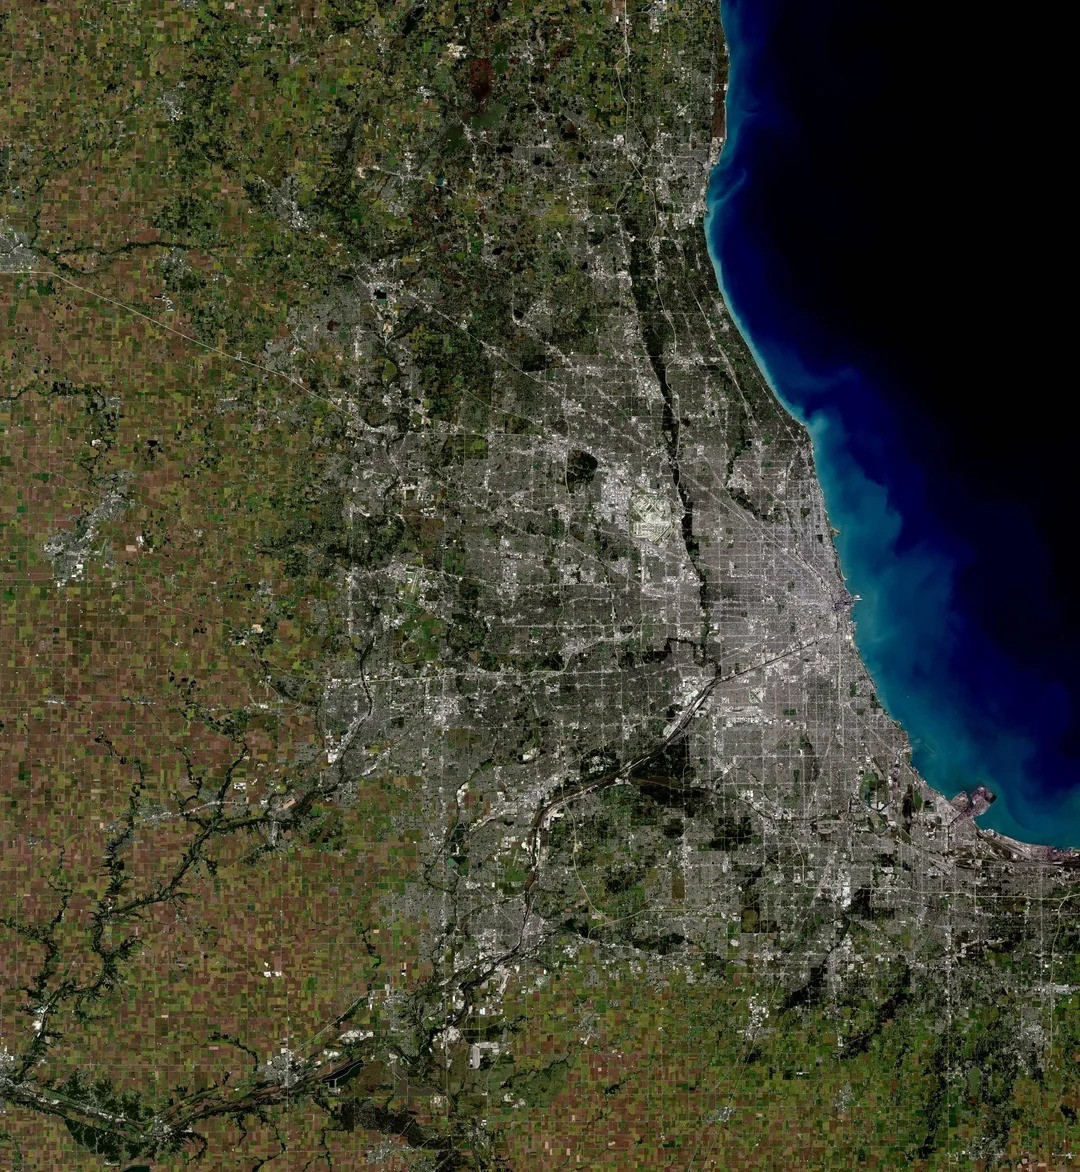
\includegraphics[width=\textwidth]{Visual/landsat.jpeg}
  \end{minipage}\hfill
  \begin{minipage}[t]{0.3\textwidth}
    \centering
    
\includegraphics[width=\textwidth]{Visual/redfin-logo-square-red-1200.png}
  \end{minipage}\hfill
  \begin{minipage}[t]{0.3\textwidth}
    \centering
    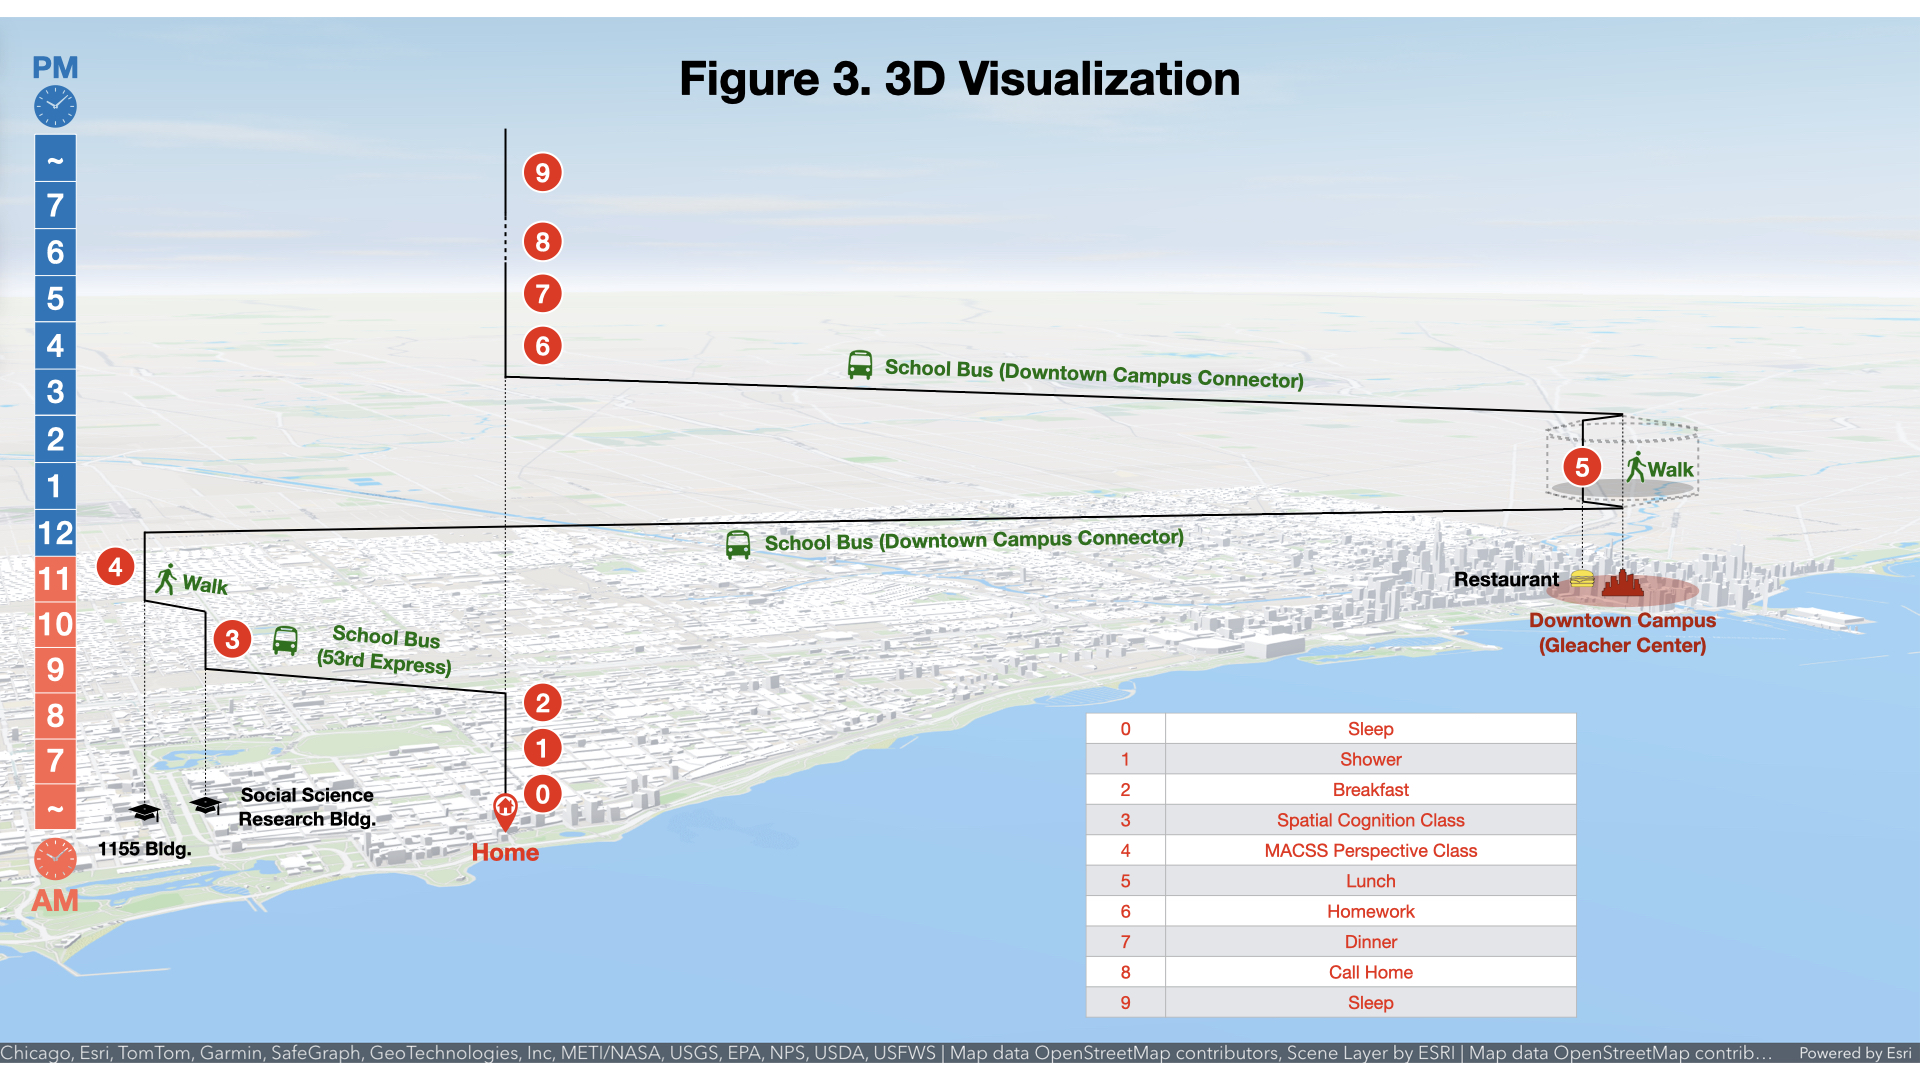
\includegraphics[width=\textwidth]{Visual/timegeo.jpeg}
  \end{minipage}
\end{figure}

\begin{table}
\centering
\begin{tabular}{|c|c|c|}
\hline
\textbf{UGS Distribution} & \textbf{Housing Price} & \textbf{Time Geography} \\
\hline
Landsat Satellite Imagery & Redfin.com & Survey Data \\
\hline
In progress & Completed & Proposed\\
\hline
\end{tabular}
\end{table}
\end{frame}

\subsection{Data Cleansing and Processing}

\begin{frame}
\frametitle{Data Cleansing and Processing}

\centering
\alert{NDVI = ((IR - R)/(IR + R))}
\begin{itemize}
    \item IR = pixel values from the infrared band
    \item R = pixel values from the red band
\end{itemize}

NDVI measures the greenness (biomass) based on satellite imagery. \textcolor{gray}{This
index calculates the contrast between two bands — the chlorophyll pigment absorption in the red band and the high reflectivity of plant material in the near-infrared (NIR) band. }

    \item A high NDVI value means rich vegetation in the area. 

    \item A moderate NDVI value means grassland and shrubs. 
    
    \item A very low NDVI means no vegetation, like ocean, cloud, or rocky areas. 
\end{frame}



\subsection{Methodology}

\begin{frame}
\frametitle{Methodology}
\begin{figure}[h]
  \centering
  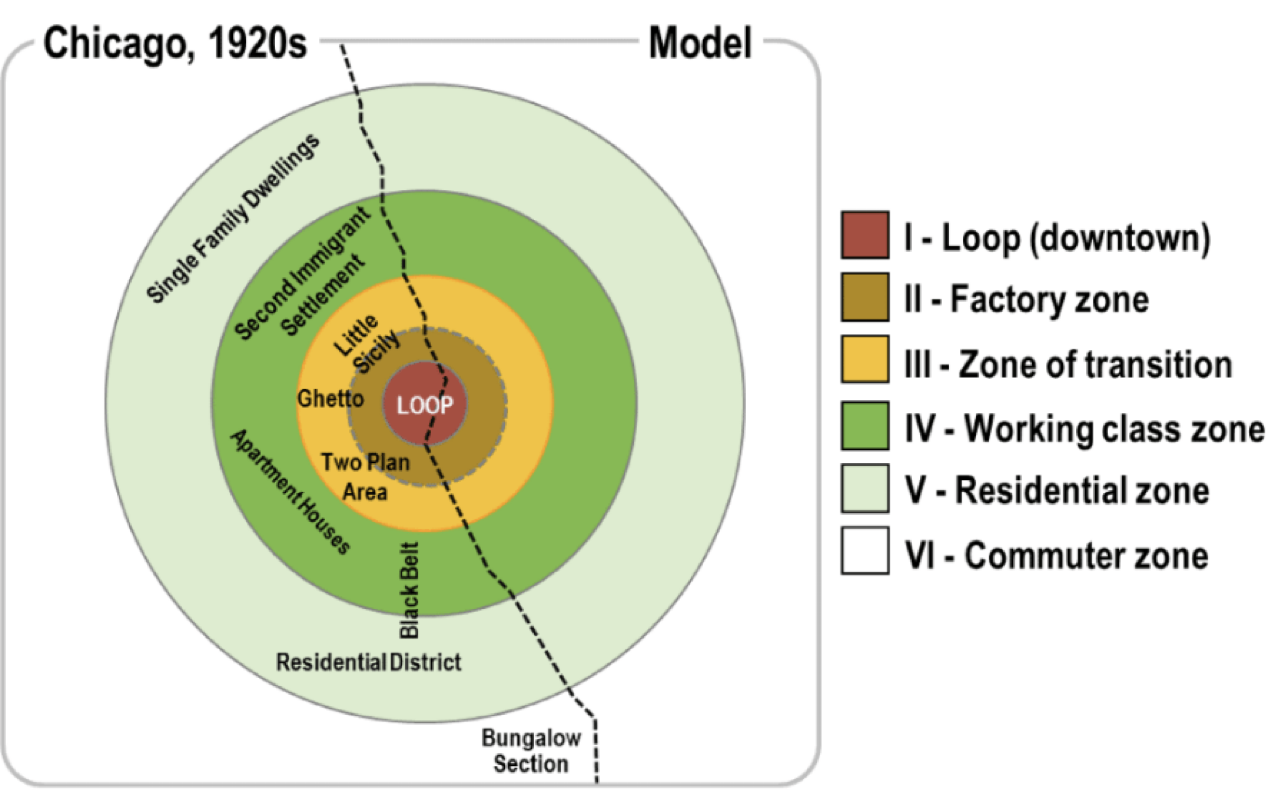
\includegraphics[width=0.55\textwidth]{Visual/concentric.jpg}
\end{figure}
For the first part of the study, I plan to compare the ML coefficients of UGS based on NDVI in housing price prediction by separately considering UGS in the city center and the city fringe. The assumption is that people show different purchasing preferences in different urban environments.

\end{frame}



\section{Conclusion}
\subsection{Initial Findings}

\begin{frame}
\frametitle{Initial Findings}
\begin{figure}[h]
  \centering
  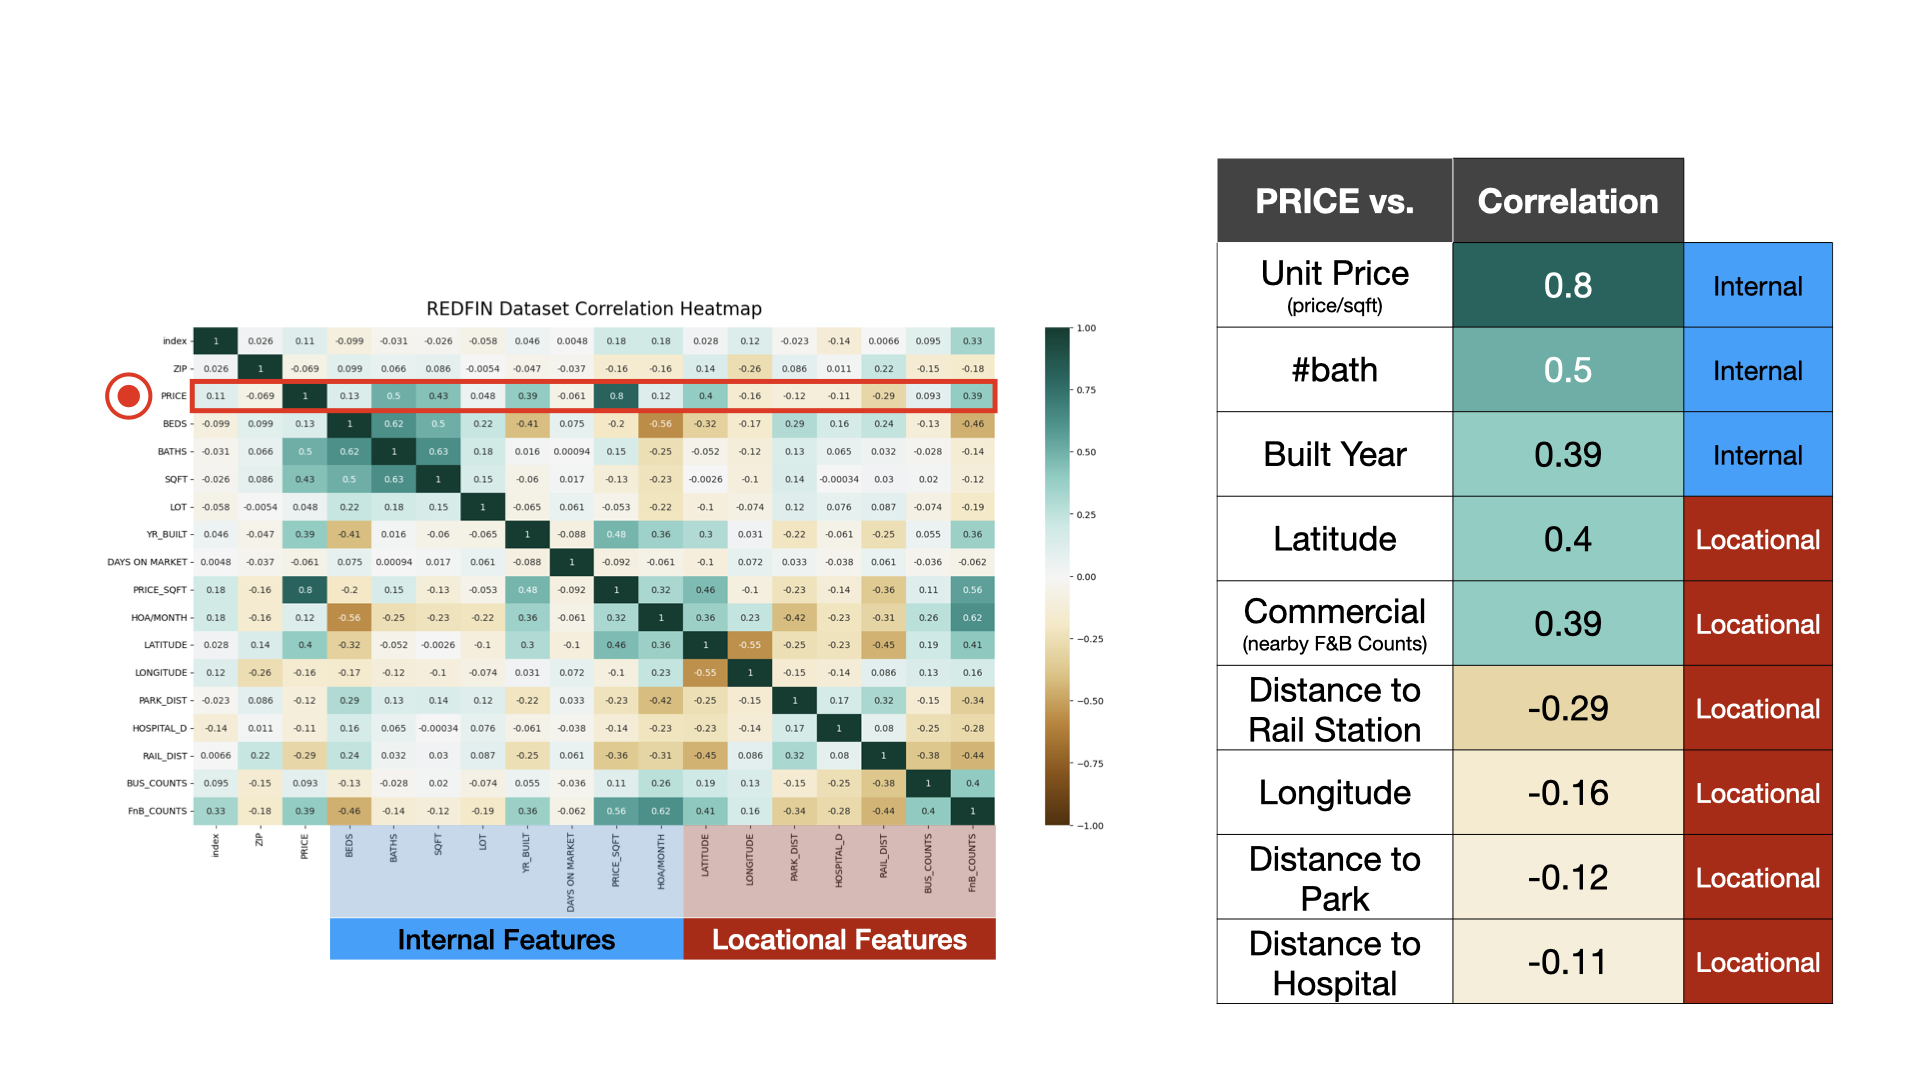
\includegraphics[width=1.0\textwidth]{Visual/heat_pre.jpeg}
\end{figure}
\end{frame}

\subsection{Feasibility}

\begin{frame}
\frametitle{Feasibility}
This project is suitable for my educational background and work experience. Professor Crystal Bae and Professor Yue Lin from the Center for Spatial Data Science can be my advisors.

This study can contribute to evaluating the economic benefits of UGS in different urban environments because the result of the pilot study and previous data collection methodology of the existing research show an underestimation of the UGS value. What is more, the time geography analysis of the research further measures if and how the residents utilize the landmark UGS differently from the tourists. The research outcome will provide a comprehensive analysis of the economic value and spatial cognitive function of UGS and can provide useful suggestions to city planners and governors on generating the most optimal economic and social benefits/outcomes with limited UGS funding. 


\end{frame}

\subsection{Timeline}

\begin{frame}
\frametitle{Timeline}
\begin{table}
\centering
\begin{tabular}{|c|c|c|}
\hline
\textbf{Task/Event} & \textbf{Time} & \textbf{Progress} \\
\hline
Redfin Data Collection & Winter 2024 & Finished \\
\hline
Satellite Imagery Data Collection & Now - Summer 2024 & En Route \\
\hline
NDVI Analysis & Summer 2024 & En Route\\
\hline
ML Model Analysis & Fall 2024 & Upcoming\\
\hline
Survey Design & Fall 2024 & Upcoming\\
\hline
Survey Conduction & Winter 2025 & Upcoming\\
\hline
\end{tabular}
\end{table}
\end{frame}

\subsection{Cost}

\begin{frame}
\frametitle{Cost}
\begin{table}
\centering
\begin{tabular}{|c|c|c|}
\hline
\textbf{Task/Event} & \textbf{Cost} & \textbf{Funding} \\
\hline
Redfin Collection & Free & N/A \\
\hline
Satellite Imagery Collection & Free/USGS & N/A\\
\hline
Survey Conduction & MTurk(200 USD) & Scholarship or JLL\\
\hline
\end{tabular}
\end{table}
\end{frame}

\begin{frame}
\frametitle{GitHub QR Code}
\begin{figure}[h]
  \centering
  
\includegraphics[width=0.55\textwidth]{Visual/qrcode_github.com.png}
\end{figure}
\end{frame}

\end{document}
